\documentclass{beamer}
\usetheme{Madrid}
\usepackage{graphicx}
\usepackage{amsmath,amssymb}
\usepackage{listings}
\usepackage{xcolor}
\lstset{
   basicstyle=\ttfamily\footnotesize,
   backgroundcolor=\color{white},
   frame=single,
   breaklines=true
}
\title{Classifying Phase Transitions with Machine Learning}
\author{Morten Hjorth-Jensen}
\date{\today}

\begin{document}

\begin{frame}
 \titlepage
\end{frame}

\begin{frame}{Outline}
 \tableofcontents
\end{frame}


\section{Introductory slides}

\begin{frame}[plain,fragile]
\frametitle{What is this talk about?}

\begin{block}{}
The main emphasis is to give you a short and pedestrian introduction to the whys and hows we can use (with several examples) machine learning methods
in physics. And why this could (or should) be of interest. 
\end{block}

\begin{block}{}
These slides and more at \href{{http://mhjensenseminars.github.io/MachineLearningTalk/doc/pub/Geiloschool/}}{\nolinkurl{http://mhjensenseminars.github.io/MachineLearningTalk/doc/pub/Geiloschool/}}
\end{block}
\end{frame}

\begin{frame}[plain,fragile]
\frametitle{Thanks to many}

Jane Kim (MSU), Julie Butler (MSU), Patrick Cook (MSU), Danny Jammooa (MSU), Daniel Bazin (MSU), Dean Lee (MSU), Witek Nazarewicz (MSU), Michelle Kuchera (Davidson College), Even Nordhagen (UiO), Robert Solli (UiO, Expert Analytics), Bryce Fore (ANL), Alessandro Lovato (ANL), Stefano Gandolfi (LANL), Francesco Pederiva (UniTN), and Giuseppe Carleo (EPFL). 
Niyaz Beysengulov and Johannes Pollanen (experiment, MSU); Zachary Stewart, Jared Weidman, and Angela Wilson (quantum chemistry, MSU)
Jonas Flaten, Oskar, Leinonen, Øyvind Sigmundson Schøyen, Stian Dysthe Bilek, and Håkon Emil Kristiansen (UiO). Marianne Bathen and Lasse Vines (experiments (UiO). Excuses to those I have omitted.
\end{frame}

\begin{frame}[plain,fragile]
\frametitle{And sponsors}

\begin{enumerate}
\item National Science Foundation, US (various grants)

\item Department of Energy, US (various grants)

\item Research Council of Norway (various grants) and my employers University of Oslo and Michigan State University
\end{enumerate}

\noindent
\end{frame}

\begin{frame}[plain,fragile]
\frametitle{AI/ML and some statements you may have heard (and what do they mean?)}

\begin{enumerate}
\item Fei-Fei Li on ImageNet: \textbf{map out the entire world of objects} (\href{{https://cacm.acm.org/news/219702-the-data-that-transformed-ai-research-and-possibly-the-world/fulltext}}{The data that transformed AI research})

\item Russell and Norvig in their popular textbook: \textbf{relevant to any intellectual task; it is truly a universal field} (\href{{http://aima.cs.berkeley.edu/}}{Artificial Intelligence, A modern approach})

\item Woody Bledsoe puts it more bluntly: \textbf{in the long run, AI is the only science} (quoted in Pamilla McCorduck, \href{{https://www.pamelamccorduck.com/machines-who-think}}{Machines who think})
\end{enumerate}

\noindent
If you wish to have a critical read on AI/ML from a societal point of view, see \href{{https://www.katecrawford.net/}}{Kate Crawford's recent text Atlas of AI}. 

\textbf{Here: with AI/ML we intend a collection of machine learning methods with an emphasis on statistical learning and data analysis}
\end{frame}

\begin{frame}[plain,fragile]
\frametitle{Types of machine learning}

\begin{block}{}
The approaches to machine learning are many, but are often split into two main categories. 
In \emph{supervised learning} we know the answer to a problem,
and let the computer deduce the logic behind it. On the other hand, \emph{unsupervised learning}
is a method for finding patterns and relationship in data sets without any prior knowledge of the system.

An important  third category is  \emph{reinforcement learning}. This is a paradigm 
of learning inspired by behavioural psychology, where learning is achieved by trial-and-error, 
solely from rewards and punishment.
\end{block}
\end{frame}

\begin{frame}[plain,fragile]
\frametitle{Main categories}

\begin{block}{}
Another way to categorize machine learning tasks is to consider the desired output of a system.
Some of the most common tasks are:

\begin{itemize}
  \item Classification: Outputs are divided into two or more classes. The goal is to   produce a model that assigns inputs into one of these classes. An example is to identify  digits based on pictures of hand-written ones. Classification is typically supervised learning.

  \item Regression: Finding a functional relationship between an input data set and a reference data set.   The goal is to construct a function that maps input data to continuous output values.

  \item Clustering: Data are divided into groups with certain common traits, without knowing the different groups beforehand.  It is thus a form of unsupervised learning.
\end{itemize}

\noindent
\end{block}
\end{frame}

\begin{frame}[plain,fragile]
\frametitle{The plethora  of machine learning algorithms/methods}

\begin{enumerate}
\item Deep learning: Neural Networks (NN), Convolutional NN, Recurrent NN, Boltzmann machines, autoencoders and variational autoencoders  and generative adversarial networks, stable diffusion and many more generative models

\item Bayesian statistics and Bayesian Machine Learning, Bayesian experimental design, Bayesian Regression models, Bayesian neural networks, Gaussian processes and much more

\item Dimensionality reduction (Principal component analysis), Clustering Methods and more

\item Ensemble Methods, Random forests, bagging and voting methods, gradient boosting approaches 

\item Linear and logistic regression, Kernel methods, support vector machines and more

\item Reinforcement Learning; Transfer Learning and more 
\end{enumerate}

\noindent
\end{frame}

\begin{frame}[plain,fragile]
\frametitle{Example of generative modeling, \href{{https://www.oreilly.com/library/view/generative-deep-learning/9781098134174/ch01.html}}{taken from Generative Deep Learning by David Foster}}

\vspace{6mm}

% inline figure
\centerline{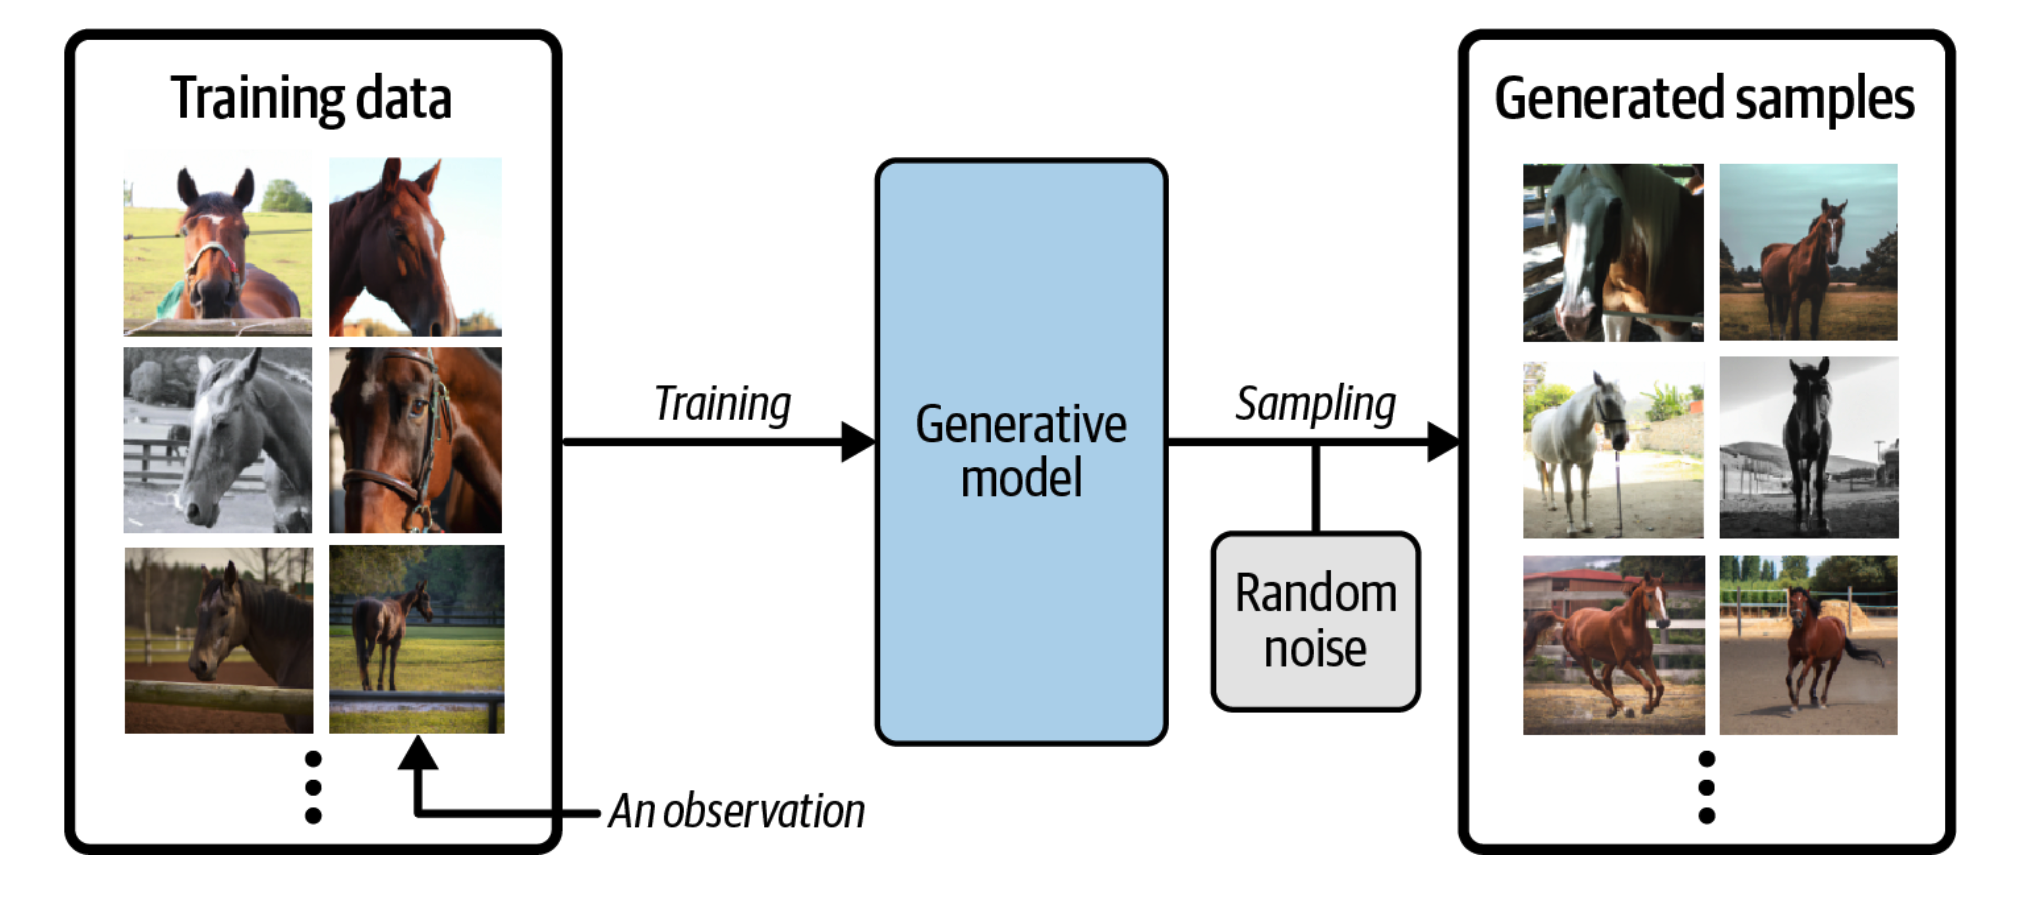
\includegraphics[width=1.0\linewidth]{figures/generativelearning.png}}

\vspace{6mm}
\end{frame}

\begin{frame}[plain,fragile]
\frametitle{Example of discriminative modeling, \href{{https://www.oreilly.com/library/view/generative-deep-learning/9781098134174/ch01.html}}{taken from Generative Deeep Learning by David Foster}}

\vspace{6mm}

% inline figure
\centerline{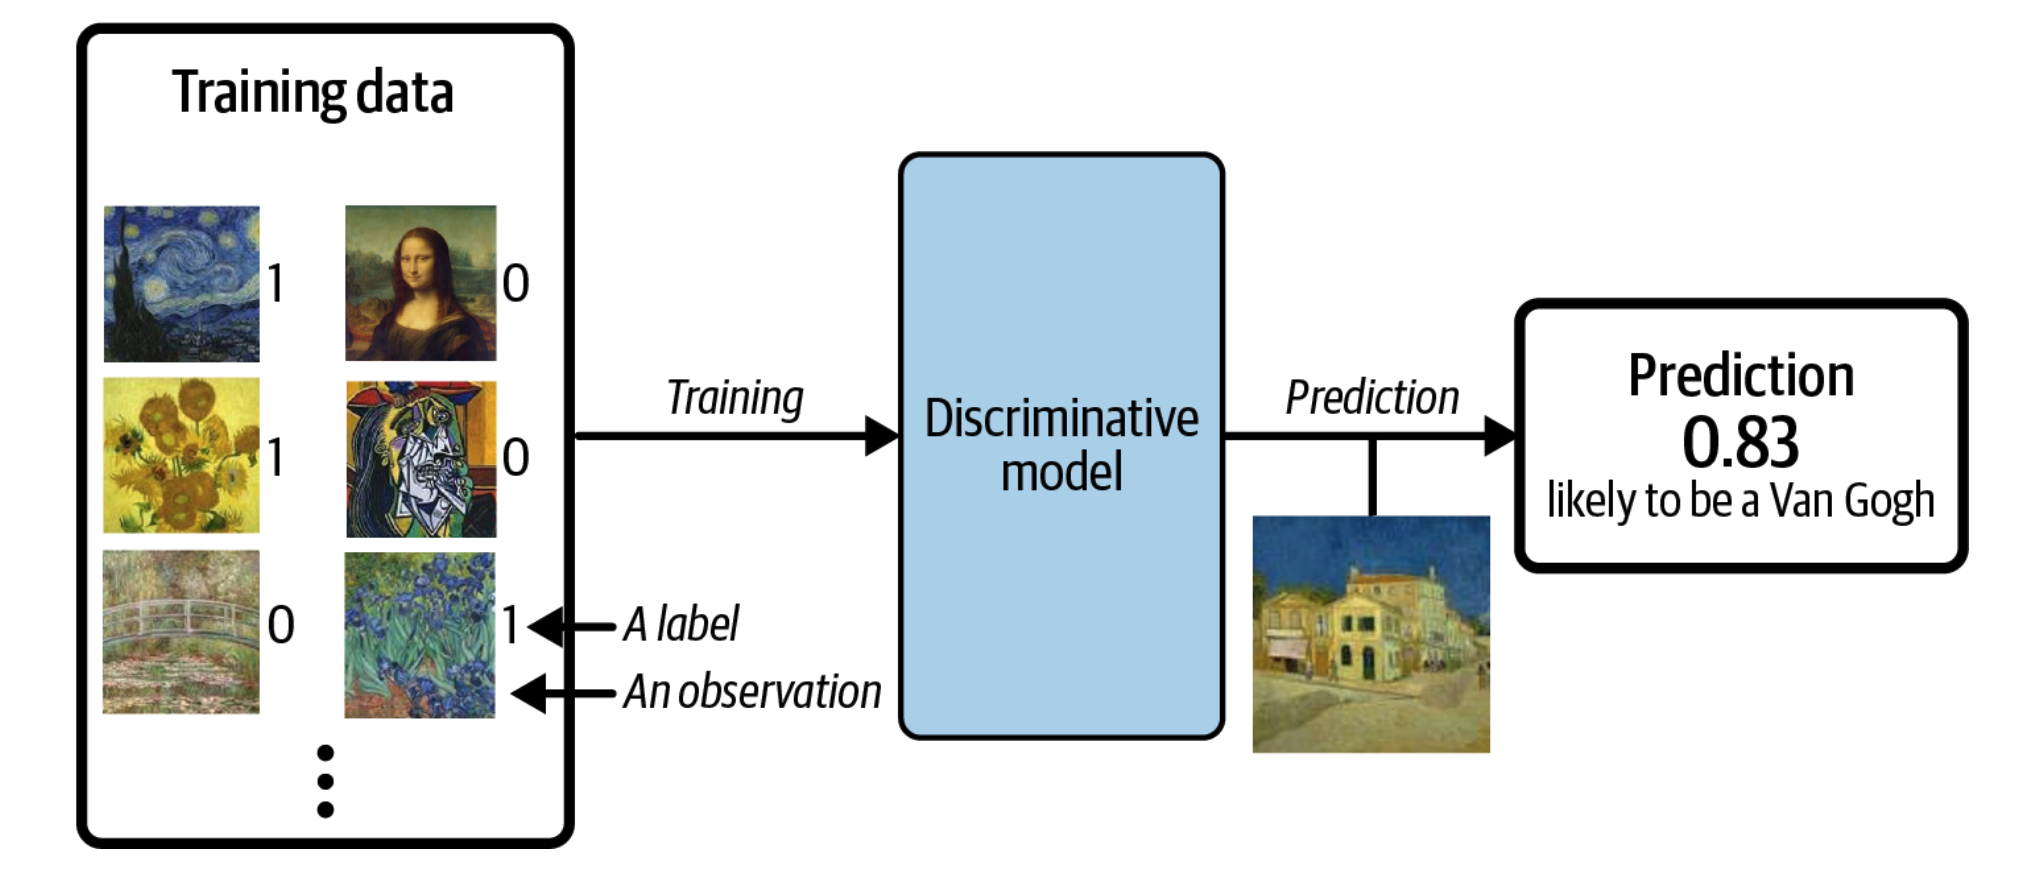
\includegraphics[width=1.0\linewidth]{figures/standarddeeplearning.png}}

\vspace{6mm}
\end{frame}

\begin{frame}[plain,fragile]
\frametitle{Taxonomy of generative deep learning, \href{{https://www.oreilly.com/library/view/generative-deep-learning/9781098134174/ch01.html}}{taken from Generative Deep Learning by David Foster}}

\vspace{6mm}

% inline figure
\centerline{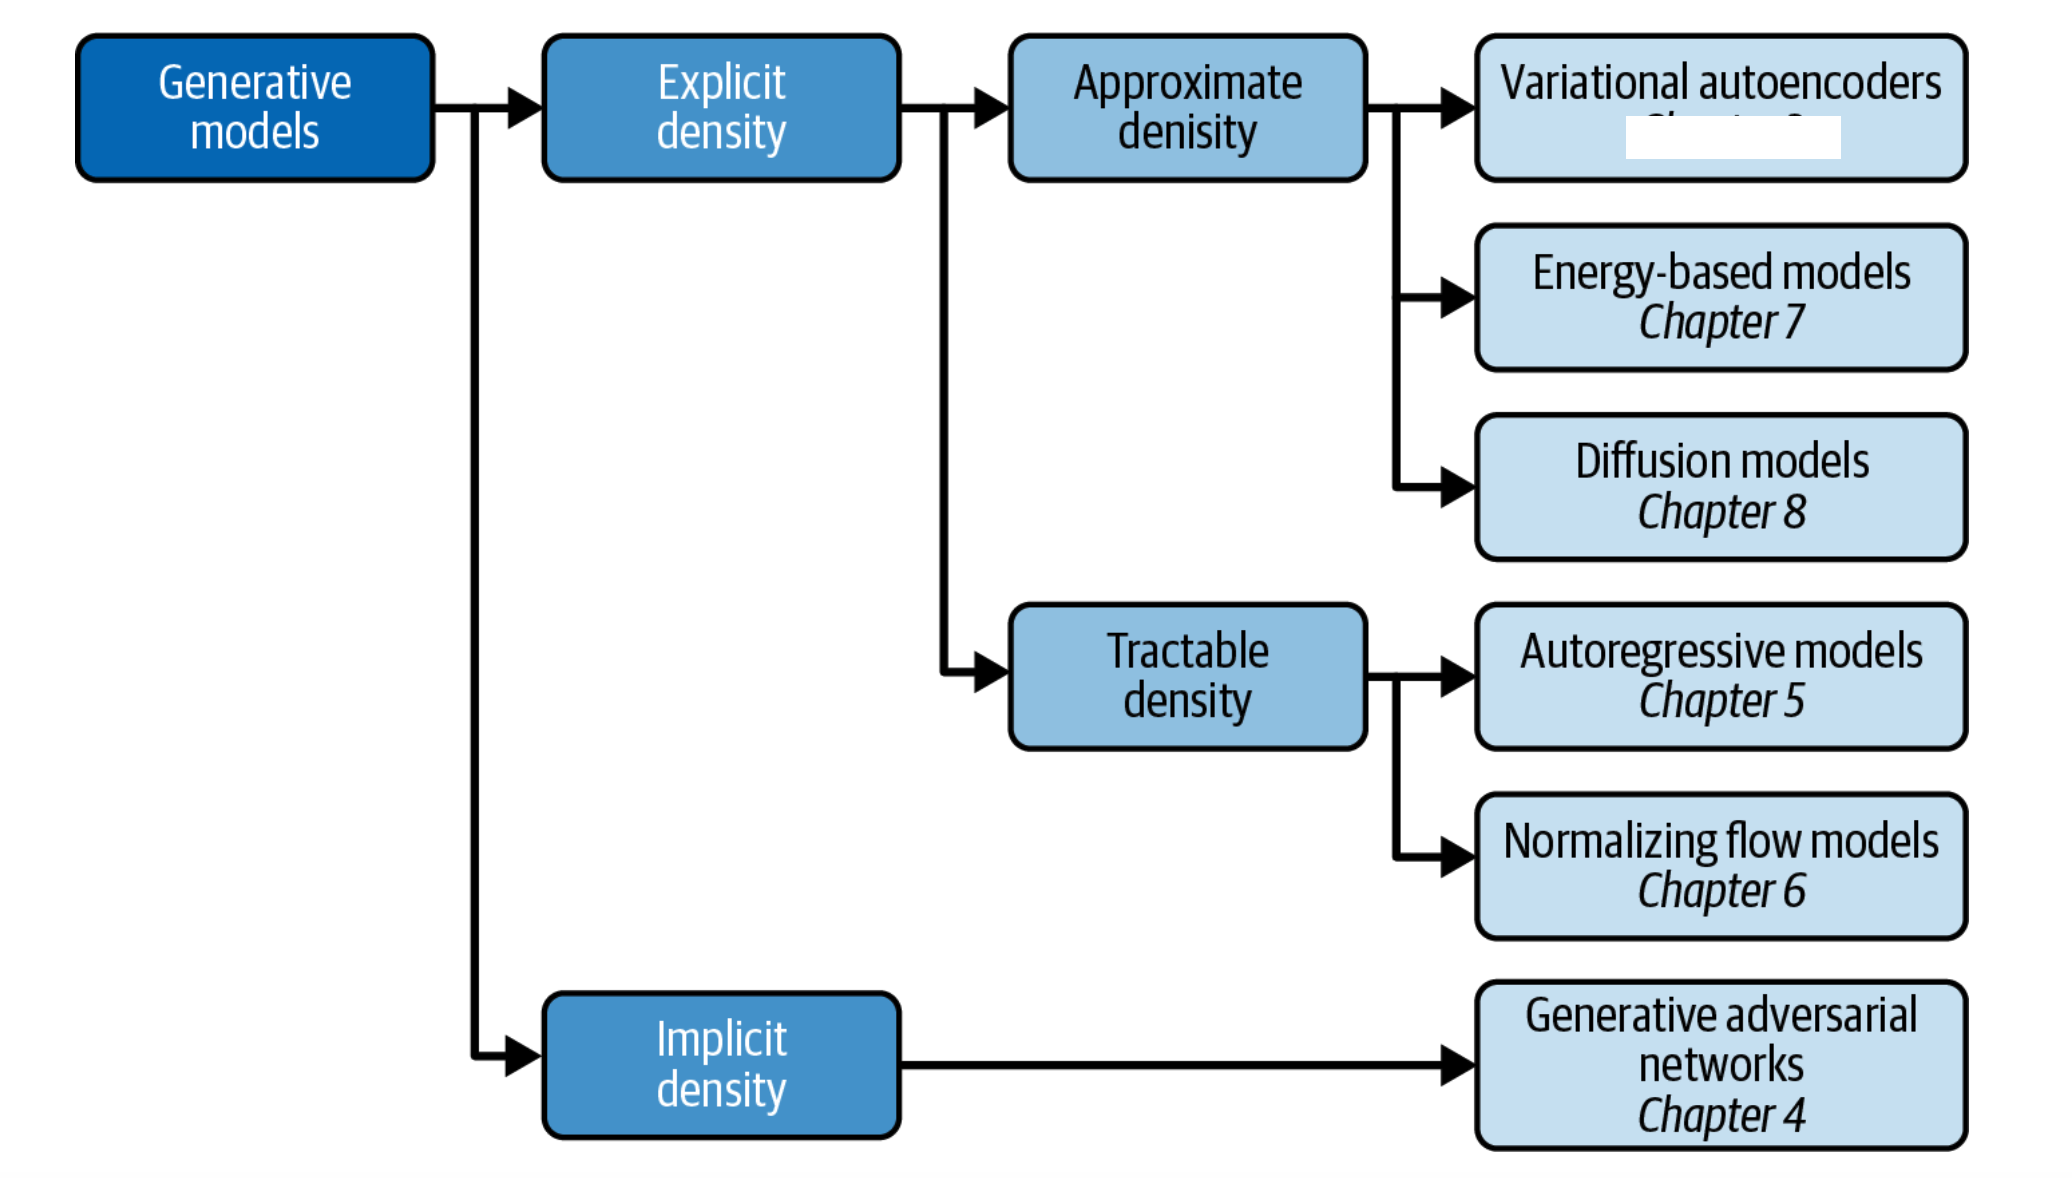
\includegraphics[width=1.0\linewidth]{figures/generativemodels.png}}

\vspace{6mm}
\end{frame}

\begin{frame}[plain,fragile]
\frametitle{Good books with hands-on material and codes}

\begin{block}{}
\begin{itemize}
\item \href{{https://sebastianraschka.com/blog/2022/ml-pytorch-book.html}}{Sebastian Rashcka et al, Machine learning with Sickit-Learn and PyTorch}

\item \href{{https://www.oreilly.com/library/view/generative-deep-learning/9781098134174/ch01.html}}{David Foster, Generative Deep Learning with TensorFlow}

\item \href{{https://github.com/PacktPublishing/Hands-On-Generative-AI-with-Python-and-TensorFlow-2}}{Bali and Gavras, Generative AI with Python and TensorFlow 2}
\end{itemize}

\noindent
\end{block}

All three books have GitHub addresses from where  one can download all codes. We will borrow most of the material from these three texts as well as 
from Goodfellow, Bengio and Courville's text \href{{https://www.deeplearningbook.org/}}{Deep Learning}
\end{frame}

\begin{frame}[plain,fragile]
\frametitle{What are the basic Machine Learning ingredients?}

\begin{block}{}
Almost every problem in ML and data science starts with the same ingredients:
\begin{itemize}
\item The dataset $\bm{x}$ (could be some observable quantity of the system we are studying)

\item A model which is a function of a set of parameters $\bm{\alpha}$ that relates to the dataset, say a likelihood  function $p(\bm{x}\vert \bm{\alpha})$ or just a simple model $f(\bm{\alpha})$

\item A so-called \textbf{loss/cost/risk} function $\mathcal{C} (\bm{x}, f(\bm{\alpha}))$ which allows us to decide how well our model represents the dataset. 
\end{itemize}

\noindent
We seek to minimize the function $\mathcal{C} (\bm{x}, f(\bm{\alpha}))$ by finding the parameter values which minimize $\mathcal{C}$. This leads to  various minimization algorithms. It may surprise many, but at the heart of all machine learning algortihms there is an optimization problem. 
\end{block}
\end{frame}

\begin{frame}[plain,fragile]
\frametitle{Low-level machine learning, the family of ordinary least squares methods}

Our data which we want to apply a machine learning method on, consist
of a set of inputs $\bm{x}^T=[x_0,x_1,x_2,\dots,x_{n-1}]$ and the
outputs we want to model $\bm{y}^T=[y_0,y_1,y_2,\dots,y_{n-1}]$.
We assume  that the output data can be represented (for a regression case) by a continuous function $f$
through
\[
\bm{y}=f(\bm{x})+\bm{\epsilon}.
\]
\end{frame}

\begin{frame}[plain,fragile]
\frametitle{Setting up the equations}

In linear regression we approximate the unknown function with another
continuous function $\tilde{\bm{y}}(\bm{x})$ which depends linearly on
some unknown parameters
$\bm{\theta}^T=[\theta_0,\theta_1,\theta_2,\dots,\theta_{p-1}]$.

The input data can be organized in terms of a so-called design matrix 
with an approximating function $\bm{\tilde{y}}$ 
\[
\bm{\tilde{y}}= \bm{X}\bm{\theta},
\]
\end{frame}

\begin{frame}[plain,fragile]
\frametitle{The objective/cost/loss function}

The  simplest approach is the mean squared error
\[
C(\bm{\Theta})=\frac{1}{n}\sum_{i=0}^{n-1}\left(y_i-\tilde{y}_i\right)^2=\frac{1}{n}\left\{\left(\bm{y}-\bm{\tilde{y}}\right)^T\left(\bm{y}-\bm{\tilde{y}}\right)\right\},
\]
or using the matrix $\bm{X}$ and in a more compact matrix-vector notation as
\[
C(\bm{\Theta})=\frac{1}{n}\left\{\left(\bm{y}-\bm{X}\bm{\theta}\right)^T\left(\bm{y}-\bm{X}\bm{\theta}\right)\right\}.
\]
This function represents one of many possible ways to define the so-called cost function.
\end{frame}

\begin{frame}[plain,fragile]
\frametitle{Training solution}

Optimizing with respect to the unknown parameters $\theta_j$ we get 
\[
\bm{X}^T\bm{y} = \bm{X}^T\bm{X}\bm{\theta},  
\]
and if the matrix $\bm{X}^T\bm{X}$ is invertible we have the optimal values
\[
\hat{\bm{\theta}} =\left(\bm{X}^T\bm{X}\right)^{-1}\bm{X}^T\bm{y}.
\]

We say we 'learn' the unknown parameters $\bm{\theta}$ from the last equation.
\end{frame}


\begin{frame}[plain,fragile]
\frametitle{Selected references}

\begin{block}{}
\begin{itemize}
\item \href{{https://arxiv.org/abs/1803.08823}}{Mehta et al.} and \href{{https://www.sciencedirect.com/science/article/pii/S0370157319300766?via%3Dihub}}{Physics Reports (2019)}.

\item \href{{https://link.aps.org/doi/10.1103/RevModPhys.91.045002}}{Machine Learning and the Physical Sciences by Carleo et al}

\item \href{{https://journals.aps.org/rmp/abstract/10.1103/RevModPhys.94.031003}}{Artificial Intelligence and Machine Learning in Nuclear Physics, Amber Boehnlein et al., Reviews Modern of Physics 94, 031003 (2022)} 

\item \href{{https://journals.aps.org/prresearch/pdf/10.1103/PhysRevResearch.5.033062}}{Dilute neutron star matter from neural-network quantum states by Fore et al, Physical Review Research 5, 033062 (2023)}

\item \href{{https://doi.org/10.48550/arXiv.2305.08831}}{Neural-network quantum states for ultra-cold Fermi gases, Jane Kim et al, Nature Physics Communcication, submitted}

\item \href{{https://doi.org/10.48550/arXiv.2305.07240}}{Message-Passing Neural Quantum States for the Homogeneous Electron Gas, Gabriel Pescia, Jane Kim et al.~arXiv.2305.07240,}

\item "Efficient solutions of fermionic systems using artificial neural networks, Nordhagen et al, Frontiers in Physics
\end{itemize}

\noindent
\end{block}
\end{frame}

\begin{frame}[plain,fragile]
\frametitle{Machine learning. A simple perspective on the interface between ML and Physics}

\vspace{6mm}

% inline figure
\centerline{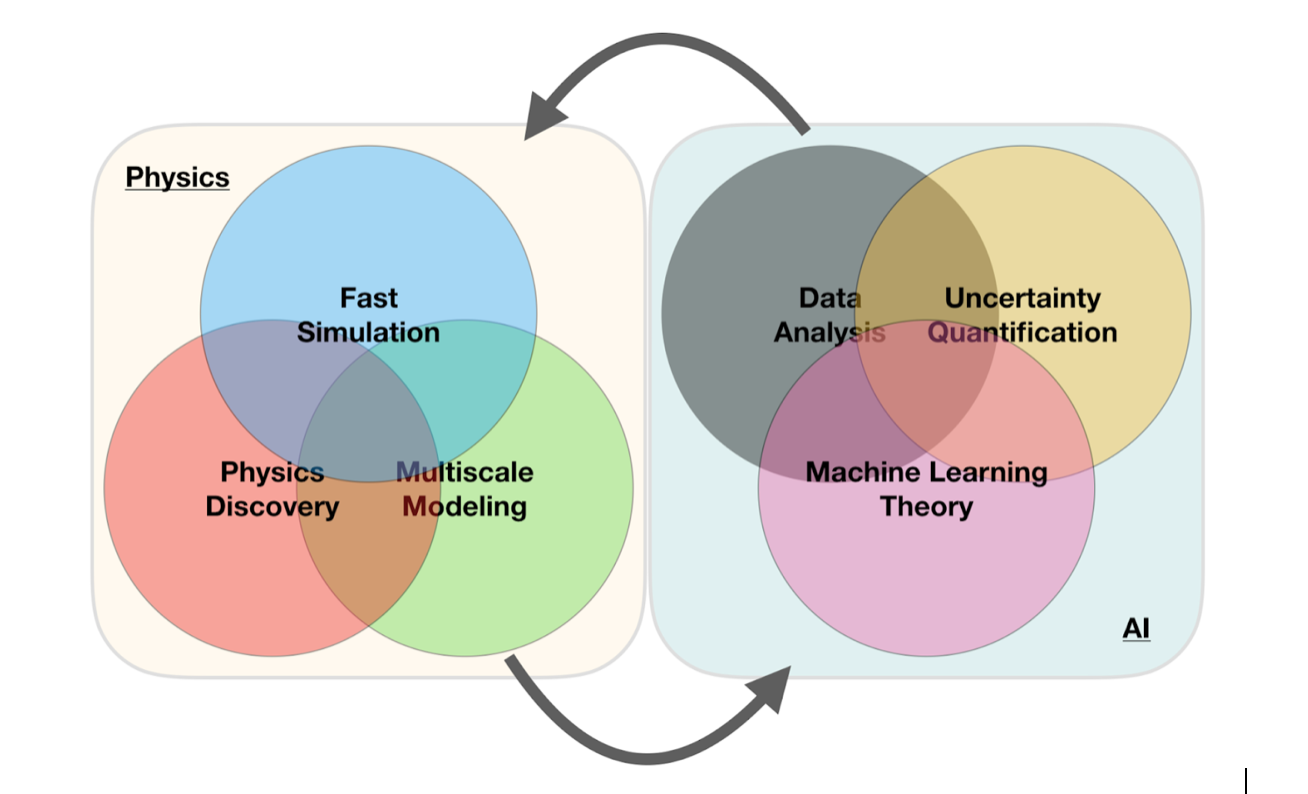
\includegraphics[width=1.0\linewidth]{figures/mlimage.png}}

\vspace{6mm}
\end{frame}

\begin{frame}[plain,fragile]
\frametitle{ML in Nuclear  Physics (or any field in physics)}

\vspace{6mm}

% inline figure
\centerline{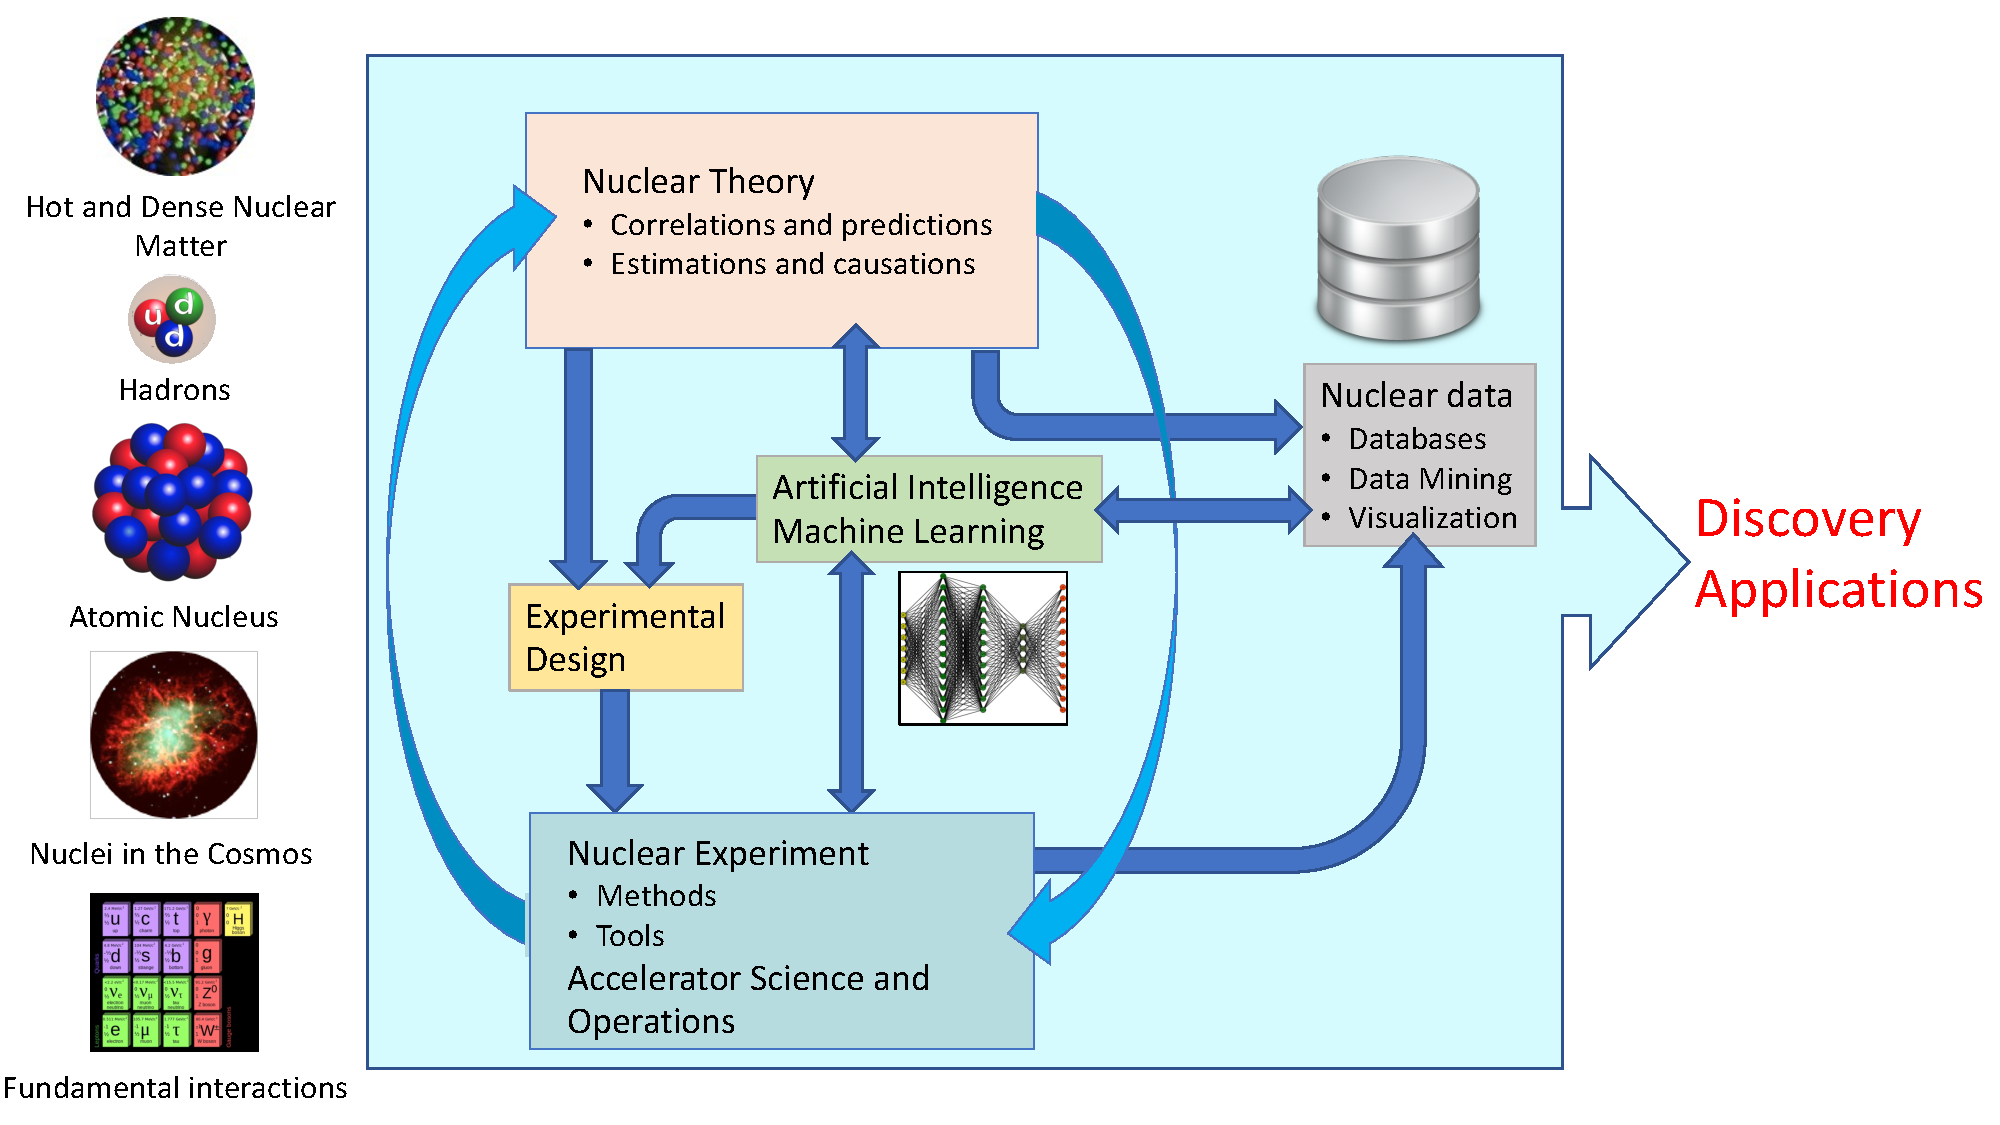
\includegraphics[width=1.0\linewidth]{figures/ML-NP.pdf}}

\vspace{6mm}
\end{frame}




\section{Phase Transitions and Critical Phenomena}

\begin{frame}{Phase Transitions: Definitions}
 \begin{itemize}
   \item A \emph{phase transition} is a qualitative change in the state of a system when a control parameter (e.g.\ temperature) passes a critical point.
   \item \textbf{Order parameter}: quantity that distinguishes phases (e.g.\ magnetization $M$ for magnetic systems).
   \item \textbf{Order vs disorder}: e.g.\ below $T_c$ a ferromagnet has $|M|>0$ (ordered), above $T_c$ $M=0$ (disordered).
   \item Phases can break symmetries; transitions can be \emph{continuous} (second-order) or \emph{first-order}.
 \end{itemize}
\end{frame}

\begin{frame}{Order Parameter \& Symmetry Breaking}
 \begin{itemize}
   \item Phase transitions often involve spontaneous symmetry breaking (e.g.\ Ising model $Z_2$ symmetry).
   \item The order parameter (e.g.\ magnetization $M = \frac{1}{N}\sum_i s_i$) changes behavior at $T_c$.
   \item In ferromagnets: $M=0$ for $T>T_c$ (symmetric paramagnet), $M\neq 0$ for $T<T_c$ (broken symmetry).
   \item Example: in 2D Ising model, two symmetric ordered states (up/down) below $T_c$.
 \end{itemize}
\end{frame}

\begin{frame}{Critical Phenomena and Scaling}
 \begin{itemize}
   \item Near a continuous transition, observables follow power laws: $M \sim |T-T_c|^\beta$, correlation length $\xi \sim |T-T_c|^{-\nu}$, etc.
   \item \textbf{Critical exponents} ($\alpha,\beta,\gamma,\nu,\dots$) characterize singular behavior.
   \item Universality: systems with the same symmetry and dimension share exponents.
   \item E.g.\ 2D Ising exponents known analytically (Onsager).
   \item At $T\to T_c$, correlation length $\xi\to\infty$, large-scale fluctuations appear.
 \end{itemize}
\end{frame}

\section{Spin Models: 2D Ising and Potts}

\begin{frame}{2D Ising Model: Definition}
 \begin{itemize}
   \item Spins $s_i = \pm 1$ on a 2D square lattice, nearest-neighbor ferromagnetic coupling.
   \item Hamiltonian:
     \[
       H = -J \sum_{\langle i,j\rangle} s_i s_j,
     \]
     with $J>0$ favoring alignment.
   \item Exhibits a second-order phase transition at critical temperature $T_c$.
   \item Order parameter: magnetization $M = \frac{1}{N}\sum_i s_i$.
   \item Below $T_c$, $M\neq0$ (ferromagnetic order); above $T_c$, $M=0$ (paramagnet).
 \end{itemize}
\end{frame}

\begin{frame}{2D Ising Model: Critical Temperature}
 \begin{itemize}
   \item Exact result (Onsager): critical point $T_c$ satisfies
     \[
       \frac{2J}{k_B T_c} = \ln(1+\sqrt{2}) \quad\Rightarrow\quad T_c \approx \frac{2J}{\ln(1+\sqrt{2})}\approx 2.269J.
     \]
     (For simplicity set $k_B=1$) 
   \item At $T>T_c$: spins are mostly disordered, no net magnetization.
   \item At $T<T_c$: long-range order develops (nonzero $M$).
   \item Correlation length $\xi$ diverges at $T_c$ 
   \item Example: at $T=T_c$ large clusters of aligned spins appear.
 \end{itemize}
\end{frame}

\begin{frame}{q-State Potts Model: Definition}
 \begin{itemize}
   \item Generalization of Ising: each spin $s_i \in \{1,2,\dots,q\}$.
   \item Ferromagnetic Potts Hamiltonian:
     \[
       H = -J \sum_{\langle i,j\rangle} \delta_{s_i,s_j},
     \]
     where $\delta_{a,b}=1$ if $a=b$, else $0$.
   \item If $q=2$, reduces to the Ising model. Higher $q$ allows richer symmetry breaking ($\mathbb{Z}_q$).
   \item Widely used to study phase transitions with multiple equivalent ordered states.
 \end{itemize}
\end{frame}

\begin{frame}{2D Potts Model: Phase Behavior}
 \begin{itemize}
   \item In 2D, the ferromagnetic Potts model has a phase transition for all $q\ge1$ 
   \item Exact critical point:
     \[
       \frac{J}{k_B T_c} = \ln\!\bigl(1+\sqrt{q}\bigr).
     \]
   \item The nature of the transition depends on $q$ 
     \begin{itemize}
       \item $1 \le q \le 4$: continuous (second-order) transition.
       \item $q > 4$: discontinuous (first-order) transition (latent heat appears).
     \end{itemize}
   \item Example: $q=3,4$ have continuous transitions; $q=5$ and higher show first-order behavior.
 \end{itemize}
\end{frame}

\section{Monte Carlo Simulation}

\begin{frame}{Monte Carlo Sampling of Spin Models}
 \begin{itemize}
   \item Use Monte Carlo (MC) to generate spin configurations at given $T$:
     sample from Boltzmann distribution $P\propto e^{-H/T}$.
   \item Metropolis algorithm: attempt random single-spin flips to equilibrate the system.
   \item Provides training data: spin configurations $\{s_i\}$ labeled by temperature or phase.
   \item Ensures statistical equilibrium and detailed balance [oai_citation:4‡rajeshrinet.github.io](https://rajeshrinet.github.io/blog/2014/ising-model/#:~:text=1,4).
   \item Efficient sampling (especially near $T_c$ cluster algorithms help, e.g.\ Wolff or Swendsen-Wang).
 \end{itemize}
\end{frame}

\begin{frame}{Metropolis Algorithm (Concept)}
 \begin{itemize}
   \item Initialize spins randomly or in a fixed state.
   \item Repeat for many steps:
     \begin{enumerate}
       \item Pick a random lattice site $i$.
       \item Propose flipping $s_i \to -s_i$ (Ising) or change state (Potts).
       \item Compute energy change $\Delta E$.
       \item If $\Delta E \le 0$, accept the flip (lower energy).
       \item Else accept with probability $\exp(-\Delta E/T)$ (Boltzmann factor) [oai_citation:5‡rajeshrinet.github.io](https://rajeshrinet.github.io/blog/2014/ising-model/#:~:text=1,4).
       \item Otherwise, reject and keep the old state.
     \end{enumerate}
   \item After equilibration, record configurations as samples.
 \end{itemize}
\end{frame}

\begin{frame}[fragile]{Metropolis Algorithm (Pseudo-code)}
 \begin{lstlisting}[language=Python]
for T in temperature_list:
   # Initialize lattice (e.g., random spins)
   config = random_configuration(Lx, Ly)
   for step in range(num_steps):
       i,j = random_site()
       dE = compute_deltaE(config, i, j)  # energy change if spin flipped
       if dE <= 0 or rand() < exp(-dE/T):
           flip_spin(config, i, j)
   record_configuration(config, T)
 \end{lstlisting}
\end{frame}

\begin{frame}{Monte Carlo Data for ML}
 \begin{itemize}
   \item Generate many spin configurations across a range of temperatures $T$.
   \item Label each configuration by its temperature or by phase (ordered/disordered).
   \item This labeled dataset is used for \emph{supervised} methods (e.g.\ CNN).
   \item For \emph{unsupervised} methods (PCA, VAE), labels are not used in training.
   \item Data augmentation: one can use symmetries (e.g.\ spin flip) to enlarge dataset.
 \end{itemize}
\end{frame}

\section{Unsupervised Learning: PCA}

\begin{frame}{Principal Component Analysis (PCA) Basics}
 \begin{itemize}
   \item PCA is an unsupervised method for dimensionality reduction.
   \item Finds orthogonal directions (principal components) of maximum variance in data.
   \item Project data onto the first few PCs to visualize structure.
   \item Advantages: linear, fast, and interpretable (PCs are linear combinations of features).
   \item Disadvantage: only captures linear correlations (may miss complex features).
 \end{itemize}
\end{frame}

\begin{frame}{PCA for Phase Identification}
 \begin{itemize}
   \item Apply PCA to the ensemble of spin configurations (flattened to vectors).
   \item The first principal component (PC1) often correlates with the order parameter (e.g.\ magnetization).
   \item Hu et al. (2017) found PCA distinguishes different phases and can locate critical points 
   \item By plotting data in the subspace of PCs, one sees separation of low-$T$ (ordered) vs high-$T$ (disordered) points.
   \item No labels needed: phase transitions are revealed by clustering in PC space 
 \end{itemize}
\end{frame}

\begin{frame}{PCA Workflow for Spin Data}
 \begin{itemize}
   \item Collect data matrix $X$ of shape (num\_samples) $\times$ (num\_features), e.g. $N\times (L\times L)$.
   \item Subtract the mean from each column (feature) of $X$.
   \item Compute covariance matrix $C = X^T X$ (or use SVD on $X$ directly).
   \item Obtain eigenvalues/vectors of $C$: $C = U \Lambda U^T$. Columns of $U$ are principal directions.
   \item Sort by eigenvalues (variance). Project $X$ onto top $k$ PCs: $X_{\rm red} = X\,U[:,1:k]$.
   \item Analyze $X_{\rm red}$: e.g.\ scatter plot PC1 vs PC2.
 \end{itemize}
\end{frame}

\begin{frame}{PCA Example: Ising Model}
 \begin{itemize}
   \item In the 2D Ising model, PC1 is essentially proportional to the overall magnetization.
   \item At $T < T_c$, configurations cluster with large positive or negative PC1 (ordered states).
   \item At $T > T_c$, configurations cluster near PC1 ≈ 0 (disordered).
   \item The variance captured by PC1 drops sharply at $T_c$, signaling the transition.
   \item PCA automatically finds these features, without knowing the physics a priori 
 \end{itemize}
\end{frame}

\begin{frame}{PCA Limitations}
 \begin{itemize}
   \item PCA is linear: complex nonlinear features (e.g.\ vortex order) may not be captured.
   \item Example: In a frustrated 2D spin model, PCA failed to detect certain correlations (vorticity) 
   \item PCA does not directly classify; it provides features for clustering or visualization.
   \item Sensitive to scaling: data should be normalized appropriately.
   \item Still useful as a first-pass: identifies the most significant variations 
 \end{itemize}
\end{frame}

\begin{frame}[fragile]{PCA with PyTorch (Example Code)}
 \begin{lstlisting}[language=Python]
import torch

# X: tensor of shape (N, L*L) containing spin configurations as floats (e.g. +1/-1)
# Center the data
X = X - X.mean(dim=0, keepdim=True)

# Compute covariance (or use torch.pca_lowrank)
cov = torch.mm(X.t(), X) / (X.size(0)-1)

# Eigen-decomposition (SVD) of covariance
U, S, V = torch.svd(cov)

# Select first k principal components
k = 2
PCs = U[:, :k]  # shape (L*L, k)

# Project data onto principal components
X_reduced = torch.mm(X, PCs)  # shape (N, k)
 \end{lstlisting}
\end{frame}

\section{Supervised Learning: CNNs}

\begin{frame}{Convolutional Neural Networks (CNNs)}
 \begin{itemize}
   \item CNNs are deep neural networks designed for spatial data (e.g.\ images).
   \item Architecture: convolutional layers (feature detectors) + pooling, followed by fully connected layers.
   \item In physics: treat spin lattice as an image with multiple channels (e.g.\ one channel of spins).
   \item CNNs can learn complex nonlinear features automatically from data.
   \item They require labeled examples for training (supervised learning).
 \end{itemize}
\end{frame}

\begin{frame}{CNN for Phase Classification}
 \begin{itemize}
   \item Prepare training data: spin configurations labeled by phase or temperature.
   \item CNN learns to map configuration $\to$ phase label (ordered/disordered) or predict $T$.
   \item As shown by Carrasquilla and Melko (2017), CNNs can identify phases from raw states 
   \item Achieves high accuracy on Ising and other models when training labels are available.
   \item CNNs exploit locality: can detect clusters or domains of aligned spins via convolution filters.
 \end{itemize}
\end{frame}

\begin{frame}{Example CNN Architecture}
 \begin{itemize}
   \item \textbf{Input}: single-channel $L\times L$ lattice (values $-1$ or $+1$).
   \item \textbf{Conv layer 1}: e.g.\ 8 filters of size $3\times3$, ReLU activation, stride=1, padding=1.
   \item \textbf{Conv layer 2}: 16 filters of size $3\times3$, ReLU, followed by a $2\times2$ max-pooling.
   \item \textbf{Fully Connected}: flatten feature maps to vector; FC layer to 64 units (ReLU); final FC to 2 outputs (softmax for binary phase).
   \item \textbf{Training}: minimize cross-entropy loss between predicted and true labels.
   \item \textbf{Note}: architecture and hyperparameters can be tuned for best performance.
 \end{itemize}
\end{frame}

\begin{frame}{CNN: Training and Results}
 \begin{itemize}
   \item Train on many labeled samples (e.g.\ temperatures $T$ and whether $T<T_c$ or $T>T_c$).
   \item The network learns features such as magnetization domains, energy patterns, etc.
   \item CNN accuracy can be very high (often $\sim$100\% on clean data) for distinguishing phases.
   \item Fukushima \& Sakai (2021): a CNN trained on 2D Ising can detect transition in $q$-state Potts 
   \item CNN behavior: at high $T$ it effectively uses average energy; at low $T$ it correlates with magnetization 
 \end{itemize}
\end{frame}

\begin{frame}{CNN Interpretability}
 \begin{itemize}
   \item CNNs are often seen as "black boxes", but their learned filters can sometimes be interpreted.
   \item Outputs correlate with known physics:
     \begin{itemize}
       \item At low $T$: classification heavily influenced by magnetization (order).
       \item At high $T$: classification influenced by internal energy (disorder) 
     \end{itemize}
   \item CNNs can generalize: e.g.\ Ising-trained CNN finds Potts $T_c$ 
   \item Visualization methods (e.g.\ saliency maps) can highlight what CNN focuses on.
 \end{itemize}
\end{frame}

\begin{frame}[fragile]{CNN (PyTorch) Code Example}
 \begin{lstlisting}[language=Python]
import torch
import torch.nn as nn
import torch.nn.functional as F

class PhaseCNN(nn.Module):
   def __init__(self, L):
       super(PhaseCNN, self).__init__()
       self.conv1 = nn.Conv2d(1, 8, kernel_size=3, padding=1)  # 1 channel -> 8
       self.conv2 = nn.Conv2d(8, 16, kernel_size=3, padding=1) # 8 -> 16
       self.pool = nn.MaxPool2d(2)  # downsample by 2
       self.fc1 = nn.Linear(16 * (L//2) * (L//2), 64)
       self.fc2 = nn.Linear(64, 2)  # 2 output classes

   def forward(self, x):
       x = F.relu(self.conv1(x))      # (B,8,L,L)
       x = self.pool(F.relu(self.conv2(x)))  # (B,16,L/2,L/2)
       x = x.view(x.size(0), -1)      # flatten
       x = F.relu(self.fc1(x))
       x = self.fc2(x)               # logits for 2 classes
       return x

# Example usage:
model = PhaseCNN(L=32)           # for a 32x32 lattice
criterion = nn.CrossEntropyLoss()
optimizer = torch.optim.Adam(model.parameters(), lr=1e-3)
 \end{lstlisting}
\end{frame}

\section{Unsupervised Learning: Variational Autoencoders}

\begin{frame}{Variational Autoencoders (VAE) Overview}
 \begin{itemize}
   \item A VAE is an \emph{unsupervised} generative model that learns a latent representation of data.
   \item Components:
     \begin{itemize}
       \item \textbf{Encoder}: maps input $X$ to parameters $(\mu, \log\sigma^2)$ of a latent Gaussian.
       \item \textbf{Latent $z$}: sampled via $z = \mu + \sigma \epsilon$ ($\epsilon\sim N(0,I)$).
       \item \textbf{Decoder}: reconstructs input $\hat{X}$ from $z$.
     \end{itemize}
   \item Loss: reconstruction error + KL divergence to enforce latent prior $\mathcal{N}(0,I)$.
   \item VAEs can both encode data compactly and generate new samples by sampling $z$.
 \end{itemize}
\end{frame}

\begin{frame}{VAE for Spin Configurations}
 \begin{itemize}
   \item Train VAE on spin configurations (no labels).
   \item Latent space (usually low-dimensional) captures key features (like order parameter).
   \item Walker et al. (2020): latent variables provide metrics to track order vs disorder in Ising 
   \item They found the latent representation closely corresponds to physical order (magnetization) 
   \item After training, one can:
     \begin{itemize}
       \item Inspect latent space (e.g.\ scatter plot of $(\mu_1,\mu_2)$) to distinguish phases.
       \item Sample $z\sim N(0,1)$ and decode to generate synthetic configurations.
     \end{itemize}
 \end{itemize}
\end{frame}

\begin{frame}{VAE Architecture Details}
 \begin{itemize}
   \item Typically use convolutional encoder/decoder for 2D structure.
   \item Example:
     \begin{itemize}
       \item Encoder: conv layers downsampling to a flat vector $\rightarrow$ linear layers $\rightarrow (\mu, \log\sigma^2)$ (size of latent space, e.g.\ 2–10 dims).
       \item Decoder: linear layer from $z$ to feature map size, followed by transposed-conv layers to reconstruct $L\times L$ lattice.
     \end{itemize}
   \item Activation: ReLU (or LeakyReLU); final output often sigmoid to model spin distribution.
   \item Training with minibatch gradient descent optimizing
     \[
       \mathcal{L} = \mathbb{E}[\|X - \hat{X}\|^2] +
       \mathrm{KL}(\mathcal{N}(\mu,\sigma)\,\|\,\mathcal{N}(0,1)).
     \]
 \end{itemize}
\end{frame}

\begin{frame}{VAE Results on Ising Model}
 \begin{itemize}
   \item The first latent dimension ($\nu_0$) learned by the VAE correlated strongly with magnetization 
   \item Plotting $\nu_0$ vs temperature shows clear change around $T_c$ (order–disorder).
   \item This means VAE "discovered" the order parameter without supervision.
   \item The VAE predicted the critical region and crossover consistently with theory 
   \item Latent space clustering: ordered-phase points separate from disordered.
 \end{itemize}
\end{frame}

\begin{frame}{VAE: Generation and Interpretation}
 \begin{itemize}
   \item After training, sample random $z$ from Gaussian prior and decode to generate configurations.
   \item The VAE latent space is continuous: can interpolate between phases.
   \item The learned representation is smooth and disentangled: one latent coordinate tracks magnetization, others track disorder.
   \item VAEs can also be used for anomaly detection: points with unusual $z$ indicate atypical states.
   \item Overall, VAEs provide both a dimensionally-reduced view of phase structure and a generative model.
 \end{itemize}
\end{frame}

\begin{frame}[fragile]{VAE (PyTorch) Code Example}
 \begin{lstlisting}[language=Python]
import torch
import torch.nn as nn
import torch.nn.functional as F

class VAE(nn.Module):
   def __init__(self, L, latent_dim=2):
       super(VAE, self).__init__()
       # Encoder: conv -> conv -> flatten -> fc_mu/fc_logvar
       self.encoder = nn.Sequential(
           nn.Conv2d(1, 8, 3, stride=2, padding=1),   # -> (8, L/2, L/2)
           nn.ReLU(),
           nn.Conv2d(8, 16, 3, stride=2, padding=1),  # -> (16, L/4, L/4)
           nn.ReLU(),
           nn.Flatten()
       )
       self.fc_mu = nn.Linear(16*(L//4)*(L//4), latent_dim)
       self.fc_logvar = nn.Linear(16*(L//4)*(L//4), latent_dim)

       # Decoder: linear -> unflatten -> convTranspose -> convTranspose
       self.decoder_fc = nn.Linear(latent_dim, 16*(L//4)*(L//4))
       self.decoder = nn.Sequential(
           nn.Unflatten(1, (16, L//4, L//4)),
           nn.ConvTranspose2d(16, 8, 3, stride=2, padding=1, output_padding=1),  # -> (8, L/2, L/2)
           nn.ReLU(),
           nn.ConvTranspose2d(8, 1, 3, stride=2, padding=1, output_padding=1),   # -> (1, L, L)
           nn.Sigmoid()
       )

   def encode(self, x):
       h = self.encoder(x)
       mu = self.fc_mu(h)
       logvar = self.fc_logvar(h)
       return mu, logvar

   def reparameterize(self, mu, logvar):
       std = torch.exp(0.5*logvar)
       eps = torch.randn_like(std)
       return mu + eps * std

   def decode(self, z):
       h = self.decoder_fc(z)
       x_recon = self.decoder(h)
       return x_recon

   def forward(self, x):
       mu, logvar = self.encode(x)
       z = self.reparameterize(mu, logvar)
       x_recon = self.decode(z)
       return x_recon, mu, logvar

# Example instantiation:
model = VAE(L=32, latent_dim=2)
optimizer = torch.optim.Adam(model.parameters(), lr=1e-3)
 \end{lstlisting}
\end{frame}

\section{Comparison of Methods}

\begin{frame}{Supervised vs Unsupervised Methods}
 \begin{itemize}
   \item \textbf{Supervised (CNN)}: Requires labeled data (phase labels or temperatures). Learns a direct mapping $\{\text{config}\}\to\{\text{phase}\}$.
   \item \textbf{Unsupervised (PCA, VAE)}: Uses only the raw configurations without labels. Learns features or representations of the data.
   \item PCA reduces dimensionality; requires no training labels 
   \item VAE learns a latent generative model; also label-free 
   \item CNN typically achieves higher accuracy in classifying known phases, but needs supervised labels.
 \end{itemize}
\end{frame}

\begin{frame}{Method Interpretability and Features}
 \begin{itemize}
   \item \textbf{PCA}: Principal components often have clear physical meaning (e.g.\ PC1 and  magnetization) 
   \item \textbf{CNN}: Filters are less directly interpretable; features are learned. However, some correlation with physics (energy, $M$) emerges 
   \item \textbf{VAE}: Latent variables can often be interpreted as order/disorder features (e.g.\ one latent ≈ magnetization) 
   \item CNN is a "black box" classifier; PCA/VAE provide insight into data structure.
   \item In terms of visualization: PCA and VAE produce low-dim plots of data (semi-transparent), whereas CNN only outputs a decision boundary.
 \end{itemize}
\end{frame}

\begin{frame}{Performance and Use Cases}
 \begin{itemize}
   \item \textbf{PCA}: Fast to compute; good for preliminary analysis of large datasets. Best for linearizable transitions.
   \item \textbf{CNN}: High classification accuracy; powerful for large and complex datasets. Can predict critical $T$ or classify multiple phases 
   \item \textbf{VAE}: Useful when no labels are available; provides a generative model. Effective in detecting transitions by latent statistics 
   \item Computational cost: PCA very cheap, CNN and VAE require training time (GPU recommended for large data).
   \item Choosing a method: depends on data availability and goal (classification vs insight vs generation).
 \end{itemize}
\end{frame}


\begin{frame}{Summary of Methods}
 \begin{itemize}
   \item \textbf{PCA}: Unsupervised, linear, interpretable. Good for dimensionality reduction and initial exploration
   \item \textbf{CNN}: Supervised, non-linear, high accuracy. Requires labels, but learns complex features (works across models 
   \item \textbf{VAE}: Unsupervised, generative. Learns latent representation reflecting order/disorder 
   \item Each method has trade-offs in accuracy, interpretability, and data requirements.
   \item Combining methods (e.g.\ using PCA or VAE features as input to another classifier) can also be fruitful.
 \end{itemize}
\end{frame}

\section{Conclusions}

\begin{frame}{Conclusions}
 \begin{itemize}
   \item Machine learning provides powerful tools for studying phase transitions in statistical models.
   \item \emph{Unsupervised} methods (PCA, VAE) can discover phase structure without labels 
   \item \emph{Supervised} methods (CNNs) achieve high classification performance given labeled data 
   \item Interpretability: PCA/VAE offer more insight into physics (latent/PC represent order parameters), while CNNs focus on prediction accuracy.
   \item Choice of method depends on the problem: data availability, need for generative modeling, and interpretability.
   \item Future directions: deeper architectures (e.g.\ ResNets), unsupervised generative flows, transfer learning across models, real experimental data.
 \end{itemize}
\end{frame}

\begin{frame}{References}
 \begin{itemize}
   \item Carrasquilla, J. \& Melko, R. G. (2017). Machine learning phases of matter. \emph{Nature Physics}, 13, 431–434 
   \item Hu, W. \textit{et al.} (2017). Discovering phases, phase transitions through unsupervised ML. \emph{Phys. Rev. E} 95, 062122 
   \item Fukushima, K. \& Sakai, K. (2021). Can a CNN trained on Ising detect Potts? \emph{Prog. Theor. Exp. Phys.} 2021, 061A01 
   \item Walker, N. \textit{et al.} (2020). 2D Ising model crossover via VAE. \emph{Sci. Rep.} 10, 13047 
   \item [Additional references on PCA, CNN, VAE methods].
 \end{itemize}
\end{frame}

\end{document}

\begin{frame}[plain,fragile]
\frametitle{Why Feed Forward Neural Networks (FFNN)?}

According to the \emph{Universal approximation theorem}, a feed-forward
neural network with just a single hidden layer containing a finite
number of neurons can approximate a continuous multidimensional
function to arbitrary accuracy, assuming the activation function for
the hidden layer is a \textbf{non-constant, bounded and
monotonically-increasing continuous function}.
\end{frame}

\begin{frame}[plain,fragile]
\frametitle{Universal approximation theorem}

The universal approximation theorem plays a central role in deep
learning.  \href{{https://link.springer.com/article/10.1007/BF02551274}}{Cybenko (1989)} showed
the following:

\begin{block}{}
Let $\sigma$ be any continuous sigmoidal function such that
\[
\sigma(z) = \left\{\begin{array}{cc} 1 & z\rightarrow \infty\\ 0 & z \rightarrow -\infty \end{array}\right.
\]
Given a continuous and deterministic function $F(\bm{x})$ on the unit
cube in $d$-dimensions $F\in [0,1]^d$, $x\in [0,1]^d$ and a parameter
$\epsilon >0$, there is a one-layer (hidden) neural network
$f(\bm{x};\bm{\Theta})$ with $\bm{\Theta}=(\bm{W},\bm{b})$ and $\bm{W}\in
\mathbb{R}^{m\times n}$ and $\bm{b}\in \mathbb{R}^{n}$, for which
\[
\vert F(\bm{x})-f(\bm{x};\bm{\Theta})\vert < \epsilon \hspace{0.1cm} \forall \bm{x}\in[0,1]^d.
\]

\end{block}
\end{frame}

\begin{frame}[plain,fragile]
\frametitle{The approximation theorem in words}

\textbf{Any continuous function $y=F(\bm{x})$ supported on the unit cube in
$d$-dimensions can be approximated by a one-layer sigmoidal network to
arbitrary accuracy.}

\href{{https://www.sciencedirect.com/science/article/abs/pii/089360809190009T}}{Hornik (1991)} extended the theorem by letting any non-constant, bounded activation function to be included using that the expectation value
\[
\mathbb{E}[\vert F(\bm{x})\vert^2] =\int_{\bm{x}\in D} \vert F(\bm{x})\vert^2p(\bm{x})d\bm{x} < \infty.
\]
Then we have
\[
\mathbb{E}[\vert F(\bm{x})-f(\bm{x};\bm{\Theta})\vert^2] =\int_{\bm{x}\in D} \vert F(\bm{x})-f(\bm{x};\bm{\Theta})\vert^2p(\bm{x})d\bm{x} < \epsilon.
\]
\end{frame}

\begin{frame}[plain,fragile]
\frametitle{More on the general approximation theorem}

None of the proofs give any insight into the relation between the
number of of hidden layers and nodes and the approximation error
$\epsilon$, nor the magnitudes of $\bm{W}$ and $\bm{b}$.

Neural networks (NNs) have what we may call a kind of universality no matter what function we want to compute.

\begin{block}{}
It does not mean that an NN can be used to exactly compute any function. Rather, we get an approximation that is as good as we want. 
\end{block}
\end{frame}

\begin{frame}[plain,fragile]
\frametitle{Class of functions we can approximate}

\begin{block}{}
The class of functions that can be approximated are the continuous ones.
If the function $F(\bm{x})$ is discontinuous, it won't in general be possible to approximate it. However, an NN may still give an approximation even if we fail in some points.
\end{block}
\end{frame}

\begin{frame}[plain,fragile]
\frametitle{Illustration of a single perceptron model and an FFNN}

\begin{figure}[!ht]  % 
  \centerline{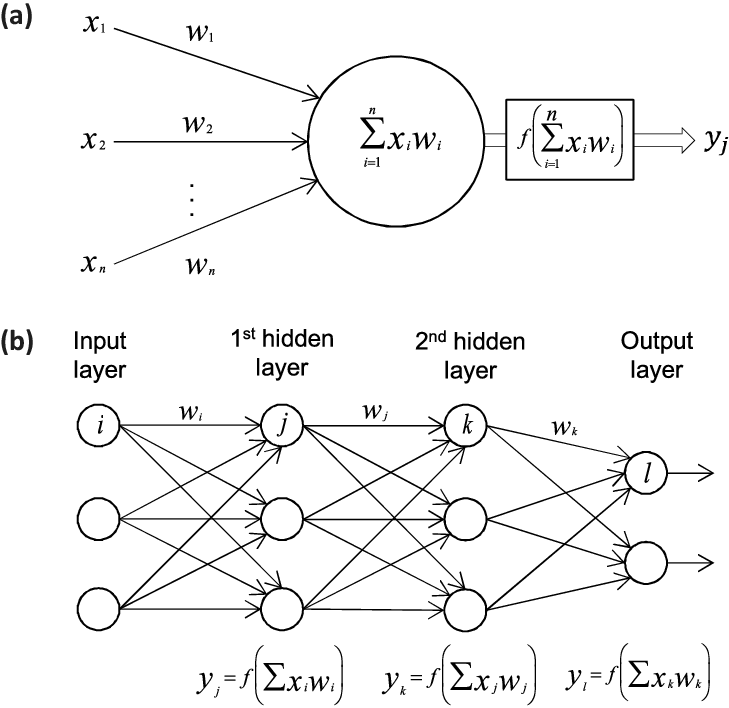
\includegraphics[width=0.7\linewidth]{figures/nns.png}}
  \caption{
  In a) we show a single perceptron model while in b) we dispay a network with two  hidden layers, an input layer and an output layer.
  }
\end{figure}
%\clearpage % flush figures
\end{frame}


